
% From using real-world datasets~\citep{deng2009imagenet} to computer games~\citep{bellemare2013arcade, tesauro1995temporal, silver2016mastering}, 
Research in artificial intelligence, and particularly deep reinforcement learning~(RL), relies on evaluating \emph{aggregate} performance on a diverse suite of tasks to assess progress. Quantitative evaluation on a suite of tasks, such as Atari games~\citep{bellemare2013arcade}, reveals strengths and limitations of methods while simultaneously guiding researchers towards methods with promising results. 
Performance of RL algorithms is usually summarized with a \emph{point estimate} of task performance measure, such as mean and median performance across tasks, aggregated over independent training runs. %Commonly used aggregate measures include . 




% To succinctly evaluate progress and measure relative performance of RL algorithms, usually \emph{point estimates} of aggregate performance, such as median performance across tasks, are reported by aggregating task performances averaged over independent runs\footnote{A run can be different from using a fixed random seed as fixing the seed may not be able to control all sources of randomness such as randomness from non-determinism of ML frameworks with GPUs. }, where each run corresponds to obtaining a result under specific random conditions, some of which might not be even controllable.

% Despite significant advances, lack of \emph{results reproducibility}~\citep{goodman2016does} is a formidable beast in deep learning~\citep[\eg][]{bouthillier2019unreproducible, beam2020challenges, musgrave2020metric}, and particularly deep RL research due to high variability in performance of RL algorithms~\citep{henderson2018deep, clary2019let, lynnerup2020survey}. 
A small number of training runs~(\figref{fig:small_runs}) coupled with high variability in performance of deep RL algorithms~\citep{henderson2018deep, mania2018simple, clary2019let, chan2019measuring, lynnerup2020survey}, often leads to substantial statistical uncertainty in reported point estimates. 
%While the lack of \emph{results reproducibility}~\citep{goodman2016does} is a challenge in deep learning~\citep{bouthillier2019unreproducible, pineau2020improving}, uncertainty in RL results exacerbates such issues. 
While evaluating more runs per task has been prescribed to reduce uncertainty and obtain reliable estimates~\citep{henderson2018deep, colas2018many, jordan2020evaluating}, 3-10 runs are prevalent in deep RL as it is often computationally prohibitive to evaluate more runs. % Although calls for %testing statistical significance of results in RL and 
% evaluating more runs have been made, % while rigorous statistical comparisons are rare. 
For example, 5 runs each on 50+ Atari 2600 games in ALE using standard protocol requires more than 1000 GPU training days~\citep{ceron2021revisiting}. As we move towards more challenging and complex RL benchmarks (\eg StarCraft~\citep{vinyals2019grandmaster}), evaluating more than a handful of runs will become increasingly demanding due to increased amount of compute and data needed to tackle such tasks. 
% For example, the number of runs has progressively dwindled over the last decades, from 1000 s in the 1998 book to 10-100 in Mountain Car-esque experiments to 3-5 in Atari games.
Additional confounding factors, such as exploration in the low-data regime, exacerbates the performance variability in deep RL -- as seen on the Atari 100k benchmark~\citep{kaiser2019model} -- often requiring many more runs to achieve negligible statistical uncertainty in reported estimates.
% Additionally, training deep RL algorithms using a limited number of samples further exacerbates their performance variability due to being far from convergence with few samples, and might require many more runs for negligible uncertainty in performance estimates.

\begin{wrapfigure}{r}{0.51\linewidth}
    \centering
    \vspace{-0.6cm}
    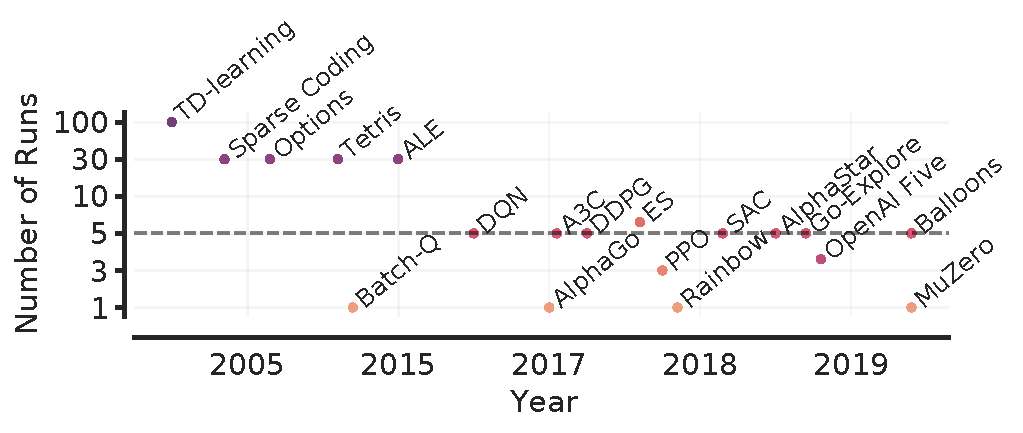
\includegraphics[width=0.99\linewidth]{new_figures/small_runs.pdf}
    \vspace{-0.65cm}
    \caption{\footnotesize{\textbf{Number of runs in RL over the years}. Beginning with DQN~\citep{mnih2015human} on the ALE, 5 or less runs are common in the field. Here, we show representative RL papers with empirical results, in the order of their publication year: TD-learning~\citep{sutton1988learning}, Sparse coding~\citep{sutton1996generalization}, Options~\citep{sutton1999between},
    Tetris~(CEM)~\citep{szita2006learning}, Batch-Q~\citep{ernst2005tree},
    ALE~\citep{bellemare2013arcade}, DQN~\citep{mnih2015human},
    AlphaGo~\citep{silver2016mastering}, A3C~\citep{mnih2016asynchronous}, DDPG~\citep{lillicrap2015continuous}, ES~\citep{salimans2017evolution},
    PPO~\citep{schulman2017proximal}, SAC~\citep{haarnoja2018soft},
    Rainbow~\citep{hessel2018rainbow}, AlphaStar~\citep{vinyals2019grandmaster}, Go-Explore~\citep{ecoffet2019go},
    OpenAI Five~\citep{berner2019dota}, Balloon navigation~\citep{bellemare2020autonomous} and MuZero~\citep{schrittwieser2020mastering}.}}
    \label{fig:small_runs}
    \vspace{-0.2cm}
\end{wrapfigure}

% a few more that may fit the claim of the paragraph,
% -hurts production environments: can lead to considering an inappropriate candidate set of algorithms in production A/B testing of RL systems
% -safety/fairness: not understanding uncertainty (when and where) can leave a decision-maker blind to poor performance in certain areas or subpopulations
% -obscures nuance in comparison: multimodal distribution of performance observed in multiple algorithms where some algorithms work better in some regimes can be hidden by point estimates

Ignoring the statistical uncertainty in deep RL results gives a false impression of fast scientific progress in the field. %whilst slowing the progress.
% often leads to unreliable and hard-to-reproduce results.
It inevitably evades the question: ``Would similar findings be obtained with new independent runs under different random conditions?''
This could steer researchers towards superficially beneficial methods~\citep{bouthillier2019unreproducible, dodge2020fine, bouthillier2021accounting}, often at the expense of better methods being neglected or even rejected early~\citep{melis2018state, lucic2017gans} as such methods fail to outperform inferior methods simply due to less favorable random conditions. Furthermore, only reporting point estimates obscures nuances in comparisons~\citep{ritter2017cognitive} and can erroneously lead the field to conclude which methods are \emph{state-of-the-art}~\citep{lin2021significant, reimers2017reporting}, ensuing wasted effort 
% and sometimes degradation in performance over existing methods 
when applied in practice~\citep{varoquaux2021failed}. Moreover, not reporting the uncertainty in deep RL results makes them difficult to reproduce except under the \emph{exact} same random conditions, %which is often impossible in practice.
which could lead to a \emph{reproducibility crisis} similar to the one that plagues other fields~\citep{ioannidis2005most, pashler2012editors, baker20161}. 
Finally, unreliable results could erode trust in deep RL research itself~\citep{rlblogpost}.%, causing broader AI research community to eschew from deep RL.

In this work, we show that recent deep RL papers compare unreliable point estimates, which are dominated by statistical uncertainty, as well as exploit non-standard evaluation protocols, using a case study on Atari 100k~(\Secref{sec:case_study}). Then, we illustrate how to reliably evaluate performance with only \emph{a handful of runs} using a more rigorous evaluation methodology that accounts for uncertainty in results~(\Secref{sec:uncertainty}).
% , which includes the use of interval estimates and performance distributions as well as efficient and robust aggregate metrics~(\Secref{sec:uncertainty}). 
To exemplify the necessity of such methodology, we scrutinize performance evaluations of existing algorithms on widely used benchmarks, including the ALE~\citep{bellemare2013arcade}~(Atari 100k, Atari 200M), Procgen~\citep{cobbe2020leveraging} and DeepMind Control Suite~\citep{tassa2018deepmind}, again revealing discrepancies in prior comparisons~(\Secref{sec:reevaluating_eval}). Our findings call for a change in how we evaluate performance in deep RL, for which we present a better methodology to prevent unreliable results from stagnating the field.

How do we reliably evaluate performance on deep RL benchmarks with only a handful of runs? As a practical solution that is easily applicable with 3-10 runs per task, we identify three statistical tools~(Table~\ref{tab:recommendations}) for improving the quality of experimental reporting. Since any performance estimate based on a finite number of runs is a \emph{random variable}, we argue that it should be treated as such. Specifically, we argue for reporting aggregate performance measures using \emph{interval estimates} via stratified bootstrap confidence intervals, as opposed to point estimates. Among prevalent aggregate measures, mean can be easily dominated by performance on a few outlier tasks, while median has high variability and zero performance on nearly half of the tasks does not change it. 
% only depends on the performance ordering across tasks and not on the magnitude of performance except at most 2 tasks. 
To address these deficiencies, we present more \emph{efficient} and \emph{robust} alternatives, such as \emph{interquartile mean}, which are not unduly affected by outliers and have small uncertainty even with a handful of runs. Furthermore, to reveal the variability in performance across tasks, we propose reporting performance distributions across all runs. Compared to prior work~\citep{bellemare2013arcade, recht-2018}, these distributions result in \emph{performance profiles}~\citep{dolan2002benchmarking} that are statistically unbiased, more robust to outliers, and require fewer runs for smaller uncertainty. 

% Specifically, we call for the use of statistical tools for estimating properties of the underlying performance 
% % Any performance metric estimated using a finite number of runs %is itself a random v
% ariable as its value
% % depends on the randomness associated with those runs.
% This implies that aggregate metrics
% can be viewed as a function of per task random variables, which itself is a random variable and 
% should be summarized and compared using \emph{interval estimates} such as bootstrap confidence intervals~\citep{eforn1979bootstrap}, as opposed to point estimates. 

%  estimators can be used to design performance metrics which are not unduly affected by outliers and have minimal uncertainty even with few runs. 

% We also show the downsides of commonly used aggregate metrics, even when used in combination with uncertainty estimates, and suggest the interquartile mean as a replacement. 



% that includes reliable interval estimates and performance distributions for reporting uncertainty and variability in results. Specifically,  we take a statistical perspective that any performance estimate based on a finite number of runs is a \emph{random variable}, as it depends on the randomness associated with those runs, and should be treated as such. %Specifically, we call for the use of statistical tools for estimating properties of the underlying performance 
% % % Any performance metric estimated using a finite number of runs %is itself a random variable as its value
% % % depends on the randomness associated with those runs.
% This implies that aggregate metrics
% % can be viewed as a function of per task random variables, which itself is a random variable and 
% should be summarized and compared using \emph{interval estimates} such as bootstrap confidence intervals~\citep{eforn1979bootstrap}, as opposed to point estimates. \emph{Efficient} and \emph{robust} statistical estimators can be used to design performance metrics which are not unduly affected by outliers and have minimal uncertainty even with few runs. To reveal the variability in performance, we propose
% comparing algorithms using their overall performance distribution across runs.
% Compared to prior work~\citep{bellemare2013arcade, recht-2018}, these distributions result in 
% \emph{performance profiles}~\citep{dolan2002benchmarking} that are  statistically unbiased, more robust to outliers, and require fewer runs for smaller uncertainty.

% Despite increasing calls to report uncertainty, e.g. via confidence intervals (Henderson et al, Chan et al), we show that this type of reporting is still rare. We also show the downsides of commonly used measures of central tendency (like the median), even when used in combination with uncertainty estimates, and suggest the interquartile mean as a replacement. We also introduce to the field new methods for reporting uncertainty, such as performance profiles

% Such comparisons result in better
% \emph{performance profiles}~\citep{dolan2002benchmarking}, a widely used tool for benchmarking optimization software. While the use of performance profiles have been suggested previously, such profiles were statistically biased and less robust to outliers as to opposed to the unbiased profiles we propose.


%and call for improvements in evaluating performance.  
% and call for a change in how we evaluate performance in deep RL, for which 
%we present a more rigorous evaluation methodology for the few-run regime to prevent the field from falling off the statistical precipice.
%Ideas:
% 
% To prevent deep reinforcement learning from plummeting into crisis, evaluation must change.  In the sections that follow, we present a more rigorous evaluation methodology that allows more meaningful comparisons to be drawn, even in the few-run regime.




\begin{table}[t]
  \centering
  \caption{\small Our recommendations for reliable evaluation, easily applicable with a handful of runs. Refer to \Secref{sec:uncertainty} for details about recommendations and \Secref{sec:reevaluating_eval} for their application to widely-used RL benchmarks.}\label{tab:recommendations}
  \vspace{0.1cm}
  \resizebox{0.94\textwidth}{!}{
  \begin{tabular}{@{}m{0.13\textwidth}m{0.39\textwidth}m{0.44\textwidth}@{}}
    \toprule
    Desideratum & Current Evaluation Protocol  & Our Recommendation \\
    \midrule
    Uncertainty in aggregate performance & 
    \textbf{Point estimates} \begin{itemize}[left=0.6em, itemsep=0.01em]  
    \item Ignore statistical uncertainty 
    \item Hinder \emph{results reproducibility} 
    \end{itemize} & Interval estimates via \hyperref[sec:stratified_bootstrap_ci]{\textbf{stratified bootstrap confidence intervals}} \\[-0.15cm]
    \midrule
    Variability in performance across tasks and runs &
    \textbf{Tables with mean scores per task} \begin{itemize}[left=0.6em, itemsep=0.01em]
        \item Overwhelming beyond a few tasks
        \item Standard deviations often omitted
        \item Incomplete picture for multimodal and heavy-tailed distributions
    \end{itemize} & 
    \hyperref[subsec:perf_profiles]{\textbf{Performance profiles}}~(\emph{score distributions}) \begin{itemize}[left=0.6em, itemsep=0.01em]
        \item Show tail distribution of scores on combined runs across tasks
        \item Allow qualitative comparisons 
        \item Easily read any score percentile
    \end{itemize} \\[-0.15cm]
    \midrule
    Aggregate metrics for summarizing performance across tasks &
    \textbf{Mean} \begin{itemize}[left=0.6em, itemsep=0.01em]
        \item Often dominated by performance on outlier tasks
    \end{itemize} 
    \textbf{Median} \begin{itemize}[left=0.6em, itemsep=0.01em]
        \item Requires large number of runs to claim improvements
        \item Poor indicator of overall performance: zero scores on nearly half the tasks do not affect it
    \end{itemize} & 
    \hyperref[sec:aggregate_metrics_robust]{\textbf{Interquartile Mean}} (IQM) across all runs \begin{itemize}[left=0.6em, itemsep=0.01em]
        \item Performance on middle 50\% of combined runs
        \item Robust to outlier scores but more statistically efficient than median
    \end{itemize}
    To show other aspects of performance gains, report average \emph{probability of improvement} and \emph{optimality gap}. \\[-0.2cm]
    \bottomrule
  \end{tabular}}
  \vspace{-0.3cm}
\end{table}